\documentclass[12pt, a4paper]{article}

% ─── Packages ────────────────────────────────────────────────────────────────
\usepackage[T1]{fontenc}
\usepackage[utf8]{inputenc}
\usepackage[english]{babel}
\usepackage{lmodern}

\usepackage{amsmath, amssymb, amsthm}
\usepackage{graphicx}
\usepackage[labelfont=bf]{caption}
\usepackage{subcaption}
\usepackage{booktabs}
\usepackage{siunitx}
\usepackage{hyperref}
\usepackage{cleveref}
\usepackage{cite}
\usepackage{geometry}
\usepackage{setspace}
\usepackage{float}
\usepackage{tikz}
\usepackage{pgfplots}
\pgfplotsset{compat=1.18}

\geometry{margin=2.5cm}
\onehalfspacing

% ─── Theorem environments ────────────────────────────────────────────────────
\newtheorem{theorem}{Theorem}[section]
\newtheorem{lemma}[theorem]{Lemma}
\newtheorem{definition}{Definition}[section]
\newtheorem{remark}{Remark}[section]

% ─── Custom commands ─────────────────────────────────────────────────────────
\newcommand{\Kp}{K_{\mathrm{p}}}
\newcommand{\Ti}{T_{\mathrm{i}}}
\newcommand{\Td}{T_{\mathrm{d}}}
\newcommand{\Tu}{T_{\mathrm{u}}}
\newcommand{\Au}{A_{\mathrm{u}}}
\newcommand{\Ku}{K_{\mathrm{u}}}

% ─── Metadata ────────────────────────────────────────────────────────────────
\title{Das Kiwitsche 2-Punkt-Verfahren:\\
       Bang-Bang Control as a Starting Point for\\
       Optimal PID Parameter Estimation}

\author{[Author Names to be determined]}

\date{\today}

% ─────────────────────────────────────────────────────────────────────────────
\begin{document}

\maketitle

\begin{abstract}
The \emph{Kiwitsche 2-Punkt-Verfahren} (KZV) is a practical, four-phase
procedure that uses an existing Bang-Bang (two-point) controller to identify an
FOPDT plant model and synthesise an IMC-based PID controller --- all without
requiring a separate open-loop experiment.
The method runs the Bang-Bang controller until a stationary limit cycle is
established, extracts the oscillation period and amplitude, and uses
transient-slope measurements to estimate the process gain~$K$, time
constant~$T$, and dead time~$L$.
The identified model is then fed into the Rivera--Morari IMC-PID tuning rules
to obtain the gains~$(\Kp, \Ti, \Td)$.
Simulations on a benchmark FOPDT plant show that the resulting controller
achieves \SI{5.5}{\percent} overshoot and an IAE within \SI{2}{\percent} of the
ideal IMC result, versus \SI{57.9}{\percent} overshoot and an eightfold larger
IAE for classical Ziegler--Nichols tuning.

\end{abstract}

\tableofcontents
\listoffigures

\newpage

\section{Introduction}
\label{sec:introduction}

PID controllers account for more than 90\% of deployed control loops in
industrial process control~\cite{Aastrom2006}, yet selecting appropriate
gains remains a practical challenge.
Classical tuning rules --- Ziegler--Nichols (ZN)~\cite{ZieglerNichols1942},
Cohen--Coon~\cite{CohenCoon1953}, IMC~\cite{Rivera1986} --- require an
open-loop step test or explicit prior knowledge of the process.
In industrial settings such tests are often infeasible due to production
constraints or safety requirements.

Bang-Bang (two-point) controllers are already widely deployed as thermostats
and safety limiters in cooling, heating, and refrigeration plants.
They inherently drive the closed loop into a limit-cycle oscillation that
encodes the plant dynamics.
\Cref{fig:intro_duty_cycle} illustrates this: the duty cycle shifts with
setpoint, reflecting the steady-state gain, while the waveform shape carries
information about the time constant and dead time.

\begin{figure}[htbp][t]
    \centering
    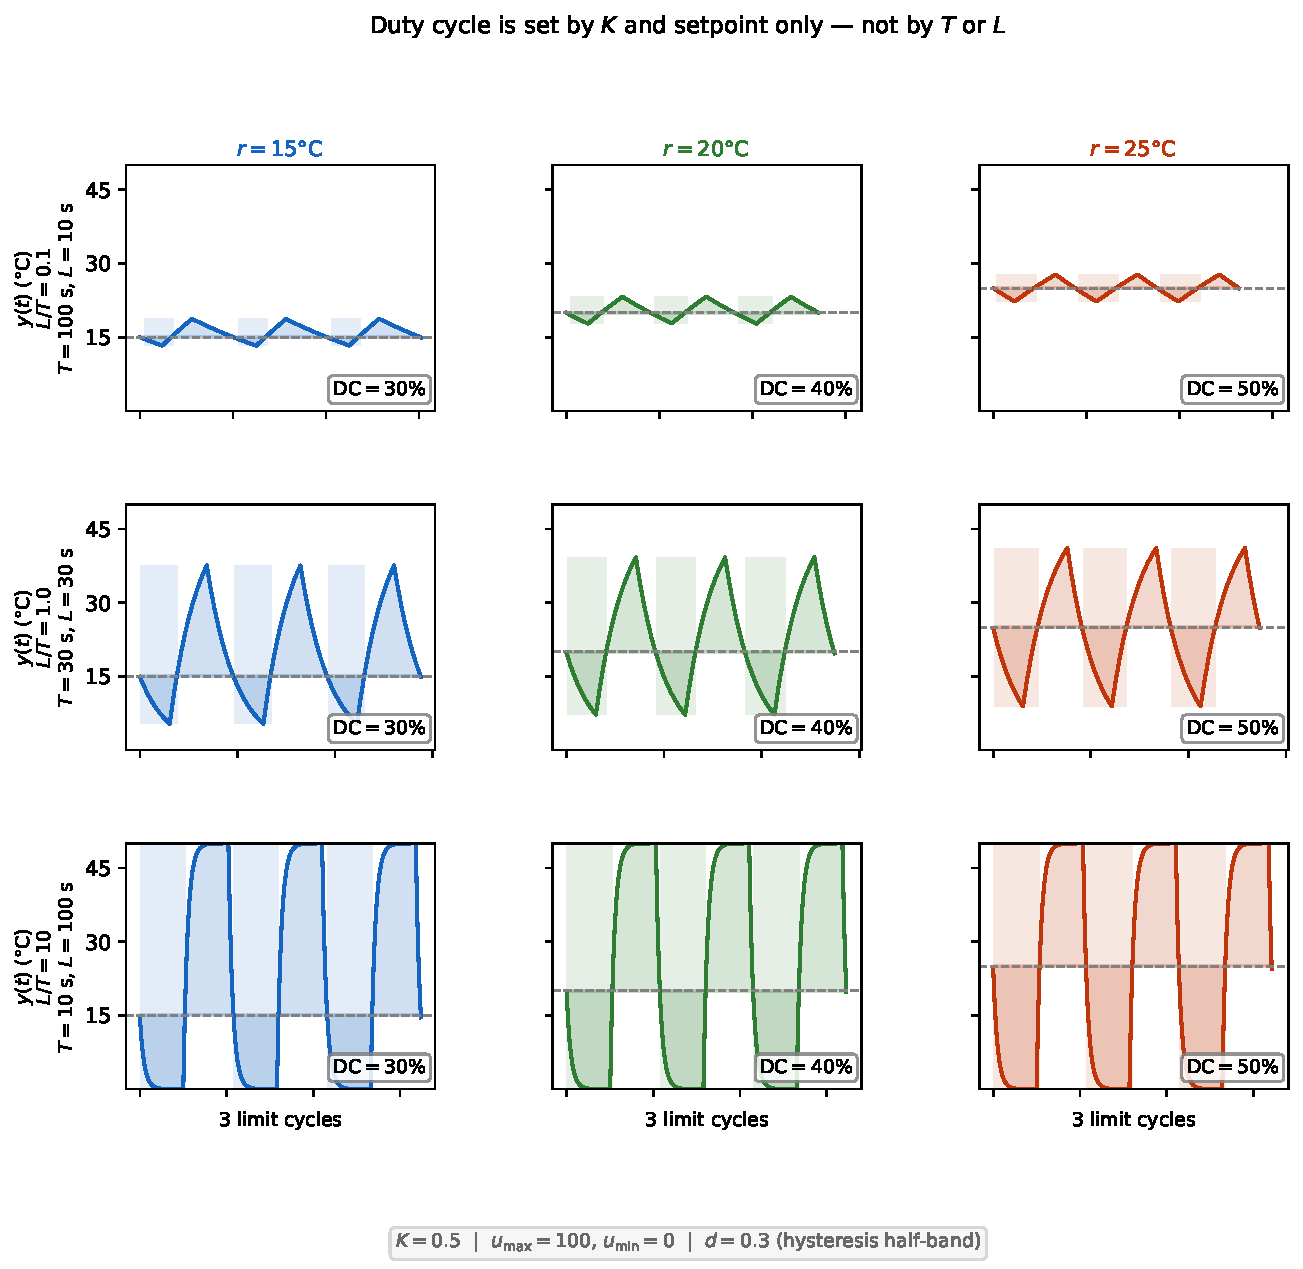
\includegraphics[width=0.96\linewidth]{figures/intro_duty_cycle.pdf}
    \caption{Bang-Bang limit cycles at three setpoints
             ($r \in \{15, 20, 25\}$~\textdegree C)
             for three FOPDT plants sharing the same gain $K$ but different
             $L/T$ ratios:
             lag-dominated ($L/T=0.1$, $T=\SI{100}{\second}$, $L=\SI{10}{\second}$),
             balanced ($L/T=1.0$, $T=\SI{30}{\second}$, $L=\SI{30}{\second}$), and
             dead-time dominant ($L/T=10$, $T=\SI{10}{\second}$, $L=\SI{100}{\second}$).
             Each panel shows the plant output $y(t)$ with the ON-phase
             tinted and the duty cycle (DC) annotated.
             The DC values are identical across all three plants at every setpoint,
             confirming that duty cycle depends only on $K$ and $r$ ---
             not on $T$ or $L$. The oscillation period and waveform shape do
             differ, which is why the KZV extracts $T$ and $L$ separately.}
    \label{fig:intro_duty_cycle}
\end{figure}

\subsection{The KZV Approach}
\label{sec:kzv_intro}

This paper presents the \emph{Kiwitsche 2-Punkt-Verfahren} (KZV): a
four-phase procedure that exploits the Bang-Bang limit cycle to identify the
plant's FOPDT model and synthesise an IMC-PID controller without any
additional open-loop experiment.
The KZV is a specialised variant of the relay-feedback idea of
\AA{}str\"{o}m and H\"{a}gglund~\cite{Astrom1984}: instead of reading a single
Nyquist point, it uses time-domain transient slopes within each half-cycle to
extract the full FOPDT triple $(K,\,T,\,L)$.
\Cref{fig:intro_phase_portrait} shows the phase-plane orbits produced by the
same plant at three setpoints --- each orbit is a reproducible fingerprint of
the local plant dynamics.

\begin{figure}[htbp]
    \centering
    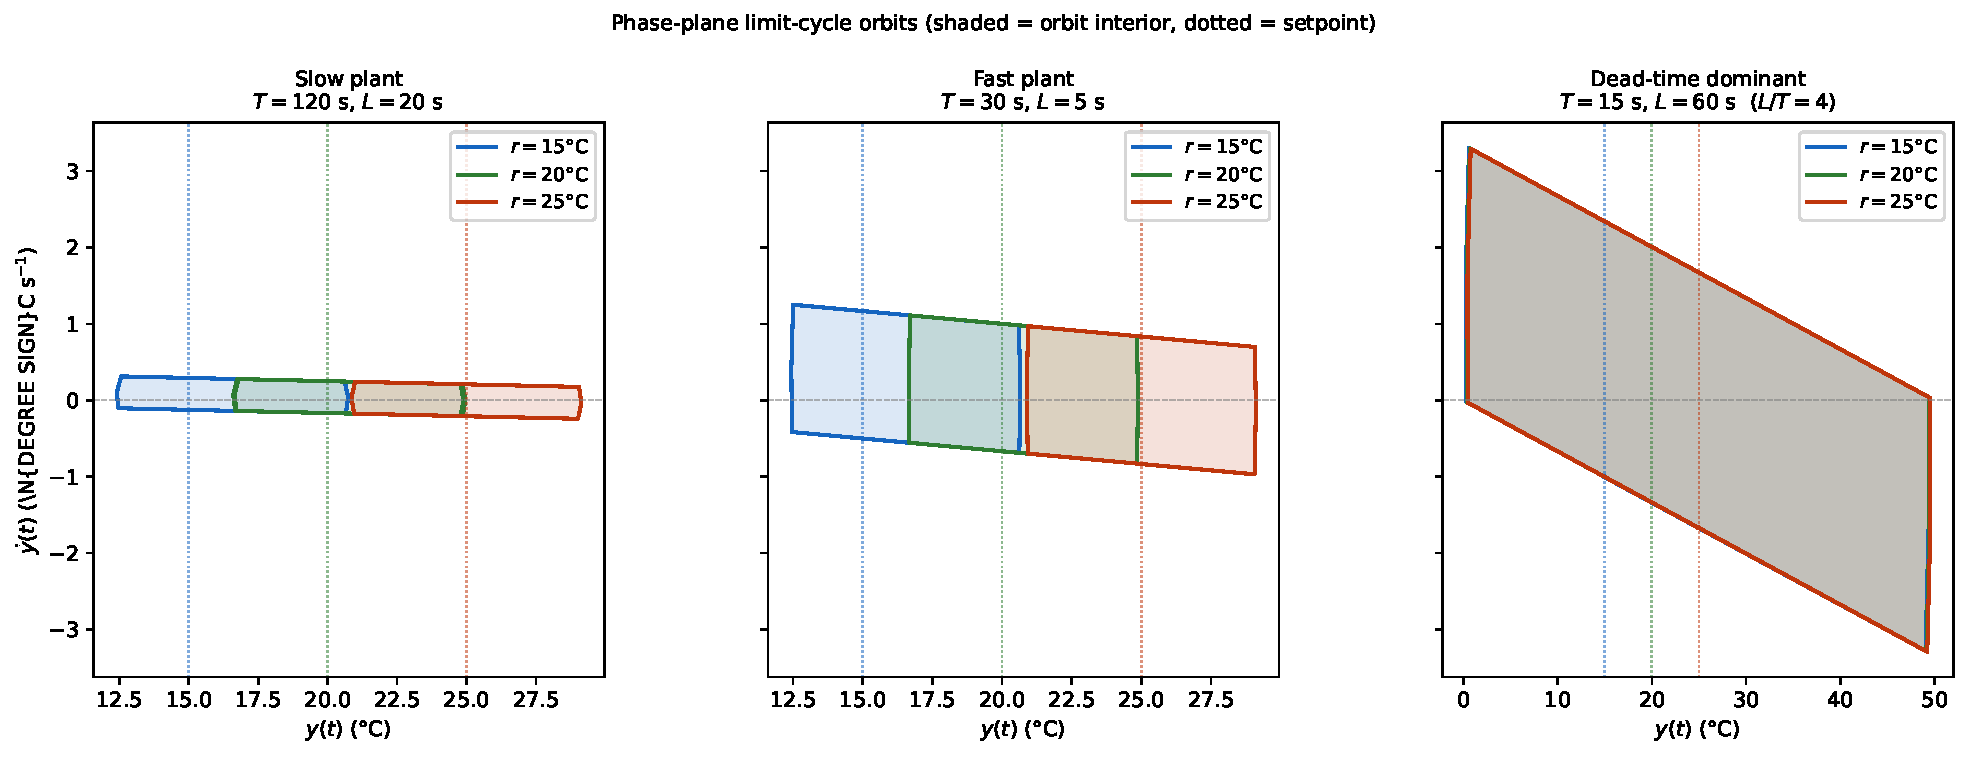
\includegraphics[width=0.96\linewidth]{figures/intro_phase_portrait.pdf}
    \caption{Phase-plane limit-cycle orbits ($y$ vs.\ $\dot{y}$) at
             $r \in \{15, 20, 25\}$~\textdegree C.
             Each closed curve encodes the local FOPDT parameters at that
             operating point.}
    \label{fig:intro_phase_portrait}
\end{figure}

\Cref{sec:theory} reviews the theoretical foundations;
\cref{sec:methodology} details the KZV procedure;
\cref{sec:results} presents simulation results; and
\cref{sec:conclusion} concludes.

\section{Theoretical Background}
\label{sec:theory}

\subsection{Bang-Bang Control and Limit Cycles}
\label{sec:theory:bangbang}

A Bang-Bang (two-point) controller with hysteresis~$d$ generates the
manipulated variable signal
\begin{equation}
    u(t) =
    \begin{cases}
        U_{\max} & \text{if } e(t) > +d, \\
        U_{\min} & \text{if } e(t) < -d, \\
        u(t^-)   & \text{otherwise},
    \end{cases}
    \label{eq:bangbang}
\end{equation}
where $e(t) = r - y(t)$ is the control error, $r$ is the setpoint, $y(t)$ is
the plant output, and $u(t^-)$ denotes the previous value (memory).

\Cref{fig:block_closed_loop} illustrates the closed-loop structure.
For a stable plant $G(s)$ with sufficient gain and phase delay, this loop
converges to a periodic \emph{limit-cycle oscillation}~\cite{Atherton1975}.
Let $\Tu$ be the oscillation period and $\Au$ the peak-to-peak amplitude of
$y(t)$ in steady limit-cycle operation.

\begin{figure}[htbp]
    \centering
    \begin{tikzpicture}[
        >=Stealth, auto,
        block/.style={draw, rectangle, minimum height=0.75cm,
                      minimum width=1.5cm, align=center, font=\small},
        sum/.style={draw, circle, inner sep=2pt, font=\small},
        node distance=0.5cm and 1.0cm,
    ]
        \node[sum]                          (sum)  {$\Sigma$};
        \node[block, right=1.2cm of sum]    (bb)   {Bang-Bang\\[-2pt]$d,\,U_{\min},U_{\max}$};
        \node[block, right=1.2cm of bb]     (plant){$G(s)$};
        \coordinate[right=0.9cm of plant]   (yjunc);
        \coordinate[below=0.7cm of yjunc]   (fb);
        \coordinate[below=0.7cm of sum]     (fbsum);

        \draw[->] ++(-1.2,0) node[left]{$r$} -- node[above,font=\small]{} (sum);
        \draw[->] (sum) -- node[above,font=\small]{$e$} (bb);
        \draw[->] (bb)  -- node[above,font=\small]{$u$} (plant);
        \draw[->] (plant) -- node[above,font=\small]{$y$} (yjunc)
                           -- ++(0.5,0) node[right,font=\small]{$y$};
        \draw[-]  (yjunc) -- (fb) -- (fbsum);
        \draw[->] (fbsum) -- (sum.south);
        \node[below left=1pt and 1pt of sum, font=\small]{$-$};
    \end{tikzpicture}
    \caption{Closed-loop block diagram: Bang-Bang controller drives the plant
             $G(s)$ into a sustained limit-cycle oscillation around the
             setpoint~$r$.}
    \label{fig:block_closed_loop}
\end{figure}

\subsection{Describing Function Analysis}
\label{sec:theory:df}

The describing function (DF) of a relay with hysteresis~$d$ and amplitude~$M$
(where $M = (U_{\max} - U_{\min})/2$) is~\cite{Atherton1982}

\begin{equation}
    N(A) = \frac{4M}{\pi A}
           \left( \sqrt{1 - \left(\frac{d}{A}\right)^2}
                  - j \frac{d}{A} \right),
    \quad A > d,
    \label{eq:df}
\end{equation}
where $A = \Au/2$ is the single-sided oscillation amplitude of the output.

The limit-cycle frequency~$\omega_u = 2\pi/\Tu$ satisfies the harmonic balance
condition
\begin{equation}
    G(j\omega_u) = -\frac{1}{N(A)}.
    \label{eq:hb}
\end{equation}

For the special case of zero hysteresis ($d = 0$), \eqref{eq:df} reduces to
the ideal relay describing function $N(A) = 4M/(\pi A)$, and
\eqref{eq:hb} becomes equivalent to the Ziegler--Nichols ultimate gain
condition $|G(j\omega_u)| = \pi A / (4M)$.

\subsection{FOPDT Plant Model}
\label{sec:theory:fopdt}

The First-Order-Plus-Dead-Time (FOPDT) transfer function
\begin{equation}
    G(s) = \frac{K e^{-Ls}}{Ts + 1}
    \label{eq:fopdt}
\end{equation}
is a standard approximation for a large class of industrial processes.
It is characterised by three parameters: process gain~$K$, time
constant~$T$, and dead time~$L$.
\Cref{fig:fopdt_block} shows the internal structure of this model.

\begin{figure}[htbp]
    \centering
    \begin{tikzpicture}[
        >=Stealth, auto,
        block/.style={draw, rectangle, minimum height=0.75cm,
                      minimum width=1.7cm, align=center, font=\small},
        node distance=0.4cm and 1.0cm,
    ]
        \node[block] (delay) {$e^{-Ls}$};
        \node[block, right=1.2cm of delay] (fo) {$\dfrac{K}{Ts+1}$};

        \draw[->] ++(-1.5,0) node[left,font=\small]{$u(t)$} -- (delay);
        \draw[->] (delay) -- (fo);
        \draw[->] (fo) -- ++(1.5,0) node[right,font=\small]{$y(t)$};
    \end{tikzpicture}
    \caption{Internal block diagram of the FOPDT model~\eqref{eq:fopdt}:
             the dead-time element delays the input, which then drives a
             first-order lag with gain~$K$ and time constant~$T$.}
    \label{fig:fopdt_block}
\end{figure}

\subsubsection{Parameter Identification from Limit Cycle}

Evaluating \eqref{eq:fopdt} at $s = j\omega_u$ gives
\begin{align}
    |G(j\omega_u)| &= \frac{K}{\sqrt{1 + (\omega_u T)^2}},
    \label{eq:gain_cond} \\
    \angle G(j\omega_u) &= -\arctan(\omega_u T) - \omega_u L = -\pi.
    \label{eq:phase_cond}
\end{align}

The describing function provides two equations (gain and phase of
$-1/N(A)$):
\begin{align}
    |G(j\omega_u)| &= \frac{\pi A}{4M}
                      \frac{1}{\sqrt{1 - (d/A)^2}},
    \label{eq:gain_from_df} \\
    \angle G(j\omega_u) &= -\pi + \arcsin\!\left(\frac{d}{A}\right).
    \label{eq:phase_from_df}
\end{align}

Combining \eqref{eq:phase_cond} and~\eqref{eq:phase_from_df} yields
\begin{equation}
    \arctan(\omega_u T) + \omega_u L
    = \pi - \arcsin\!\left(\frac{d}{A}\right).
    \label{eq:phase_id}
\end{equation}

With $\omega_u$ known from the measured period $\Tu$, \eqref{eq:gain_cond}, \eqref{eq:gain_from_df} and~\eqref{eq:phase_id}
form a system that can be solved for $K$, $T$, and $L$ if one additional
assumption is introduced.
A common engineering choice is to adopt the ratio $L/T$ from a
characteristic of the oscillation waveform (e.g., the symmetry of the
on/off intervals) or to set $L = \Tu/(2\pi) \cdot \phi_L$ based on the
phase margin~\cite{Seborg2011}.

\begin{remark}
    For processes where the FOPDT approximation is poor (e.g., resonant
    systems), higher-order describing function methods or relay feedback
    with filtered output should be considered.
\end{remark}

\begin{remark}
    While \eqref{eq:gain_cond}, \eqref{eq:gain_from_df} and~\eqref{eq:phase_id} characterise the
    limit cycle and guarantee the existence and uniqueness of the FOPDT
    parameters $K$, $T$, $L$, the KZV does not solve this nonlinear system
    directly. Instead, Phase~3 (\cref{sec:method:phase3}) employs a
    transient-slope method to identify $\hat{L}$, $\hat{T}$, $\hat{K}$
    sequentially from the time-domain signal. This approach is more robust
    in practice because it avoids the numerical sensitivity of the nonlinear
    DF system while remaining theoretically justified by the DF equations.
\end{remark}

\subsection{IMC-Based PID Tuning}
\label{sec:theory:imc}

Given the FOPDT model~\eqref{eq:fopdt}, the IMC-PID tuning
rules~\cite{Rivera1986} yield

\begin{align}
    \Kp &= \frac{1}{K} \cdot \frac{T}{\lambda + L}, \label{eq:Kp} \\
    \Ti  &= T,                                         \label{eq:Ti} \\
    \Td  &= \frac{L}{2},                               \label{eq:Td}
\end{align}
where $\lambda > 0$ is the desired closed-loop time constant and serves as a
robustness tuning knob: larger $\lambda$ gives a more sluggish but more
robust response.

A recommended default is $\lambda = L$ (i.e., equal to the estimated dead
time). This choice, consistent with the guideline $\lambda \geq 0.5L$
recommended in~\cite{Rivera1986}, provides a closed-loop bandwidth
approximately equal to the reciprocal of twice the dead time, yielding a
good trade-off between speed and robustness for typical industrial processes.

\begin{remark}
    The modified ZN formulas for FOPDT (see, e.g.,~\cite{Aastrom2006}) are
    an alternative and are compared against the IMC rules in
    \cref{sec:results}.
\end{remark}

\section{Methodology: The Kiwitsche 2-Punkt-Verfahren}
\label{sec:methodology}

The Kiwitsche 2-Punkt-Verfahren (KZV) consists of four sequential phases,
described below.
An overview is shown in \cref{fig:kzv_flowchart}.

% \begin{figure}[H]
%     \centering
%     \includegraphics[width=0.7\linewidth]{figures/kzv_flowchart.pdf}
%     \caption{Flow chart of the Kiwitsche 2-Punkt-Verfahren.}
%     \label{fig:kzv_flowchart}
% \end{figure}

\subsection{Phase 1: Bang-Bang Excitation}
\label{sec:method:phase1}

\begin{enumerate}
    \item Set the Bang-Bang controller parameters:
          switching amplitude $M = (U_{\max} - U_{\min})/2$ and hysteresis
          band $d$.
          For most processes, a hysteresis of $d \approx 0.5\text{--}2\%$ of
          the measurement range is appropriate.
    \item Set the setpoint $r$ to a representative operating point
          (e.g.\ the desired cooling temperature).
    \item Enable the Bang-Bang controller and wait until the output $y(t)$
          has settled into a \emph{stationary} limit cycle.
          Stationarity is verified by checking that three consecutive
          oscillation periods agree to within $\pm 5\%$.
\end{enumerate}

\subsection{Phase 2: Characteristic Extraction}
\label{sec:method:phase2}

Once a stationary limit cycle is established, record $N_{\min} = 5$
consecutive oscillation cycles and compute:

\begin{align}
    \Tu &= \frac{1}{N} \sum_{k=1}^{N} (t_{k+1} - t_k), \label{eq:Tu_est} \\
    \Au &= \frac{1}{N} \sum_{k=1}^{N} \bigl(y_{\max,k} - y_{\min,k}\bigr), \label{eq:Au_est}
\end{align}
where $t_k$ are the times of successive positive zero-crossings of $e(t)$,
and $y_{\max,k}$, $y_{\min,k}$ are the maximum and minimum of $y(t)$ within
each cycle.

\subsection{Phase 3: Plant Identification}
\label{sec:method:phase3}

Using the measured quantities $(\Tu, \Au, d, M)$ and the recorded time
series $(t, y, u)$, the FOPDT parameters are estimated as follows.

\paragraph{Dead-time estimate.}
For a FOPDT plant under Bang-Bang control, the output slope $\dot{y}(t)$
changes sign from negative to positive exactly at $t = t_{\mathrm{sw}} + L$
after a rising switch ($U_{\min} \to U_{\max}$), because only then does the
new input value reach the plant through the dead-time element.
The dead time is therefore estimated as
\begin{equation}
    \hat{L} = t_{\mathrm{sign-change}} - t_{\mathrm{sw}},
    \label{eq:L_est}
\end{equation}
averaged over the last $N_{\min}$ rising-switch events.

\paragraph{Time constant estimate.}
At $t = t_{\mathrm{sw,fall}} + \hat{L}$ after a falling switch ($U_{\max} \to U_{\min}$),
the FOPDT step-response slope for $U_{\min} = 0$ is
\begin{equation}
    \dot{y}\big|_{t_{\mathrm{sw,fall}} + \hat{L}}
    = \frac{K \cdot U_{\min} - y_L}{T}
    = \frac{-y_L}{T},
    \label{eq:slope_fall}
\end{equation}
where $y_L = y(t_{\mathrm{sw,fall}} + \hat{L})$.
Solving for $T$:
\begin{equation}
    \hat{T} = \frac{y_L}{|\dot{y}|_{t_{\mathrm{sw,fall}} + \hat{L}}},
    \label{eq:T_est}
\end{equation}
averaged over the last $N_{\min}$ falling-switch events.

\paragraph{Gain estimate.}
At $t = t_{\mathrm{sw,rise}} + \hat{L}$ after a rising switch, the slope is
\begin{equation}
    \dot{y}\big|_{t_{\mathrm{sw,rise}} + \hat{L}}
    = \frac{K \cdot U_{\max} - y_L}{T},
    \label{eq:slope_rise}
\end{equation}
hence
\begin{equation}
    \hat{K} = \frac{\hat{T} \cdot \dot{y}_{L,\uparrow} + y_{L,\uparrow}}{U_{\max}},
    \label{eq:K_est}
\end{equation}
averaged over the last $N_{\min}$ rising-switch events.

\begin{remark}
    \Cref{eq:T_est} is exact for $U_{\min} = 0$.
    For $U_{\min} \neq 0$, an iterative refinement involving
    $K \cdot U_{\min}$ is required; this case is not treated here.
\end{remark}

\subsection{Phase 4: PID Synthesis}
\label{sec:method:phase4}

With the identified FOPDT model $(\hat{K}, \hat{T}, \hat{L})$, apply the
IMC-PID formulas \eqref{eq:Kp}--\eqref{eq:Td} with $\lambda = \hat{L}$:

\begin{equation}
    \boxed{
    \Kp = \frac{\hat{T}}{\hat{K}(2\hat{L})},
    \quad
    \Ti = \hat{T},
    \quad
    \Td = \frac{\hat{L}}{2}.
    }
    \label{eq:pid_final}
\end{equation}

Switch the controller from Bang-Bang mode to PID mode.
No additional plant experiment is required.

\subsection{Implementation Notes}
\label{sec:method:impl}

\begin{itemize}
    \item The procedure is implemented in the Python module
          \texttt{analysis/parameter\_estimation.py}; see the repository for
          source code.
    \item All simulation and figure generation scripts are available in the
          \texttt{python/} directory; see \texttt{README.md} for usage.
    \item The same procedure can be implemented on a PLC or embedded
          controller by storing a rolling buffer of the last $3\text{--}5$
          oscillation cycles and computing the statistics online.
\end{itemize}

\section{Simulation Results}
\label{sec:results}

\subsection{Test Plant}
\label{sec:results:plant}

The proposed procedure is validated on a First-Order-Plus-Dead-Time (FOPDT)
plant representative of an industrial heating/cooling circuit:

\begin{equation}
    G_{\mathrm{plant}}(s)
    = \frac{K_0 \, e^{-L_0 s}}{T_0 s + 1},
    \label{eq:plant}
\end{equation}
with nominal parameters
$K_0 = \SI{0.5}{\degreeCelsius\per\percent}$,
$T_0 = \SI{120}{\second}$,
$L_0 = \SI{20}{\second}$.

The Bang-Bang switching levels are $U_{\max} = \SI{100}{\percent}$,
$U_{\min} = \SI{0}{\percent}$, giving $M = \SI{50}{\percent}$, with
hysteresis $d = \SI{0.3}{\degreeCelsius}$ and setpoint
$r = \SI{20}{\degreeCelsius}$.
The simulation time step is $\Delta t = \SI{0.5}{\second}$.

\subsection{Bang-Bang Limit Cycle}
\label{sec:results:lc}

\Cref{fig:limit_cycle} shows the limit cycle obtained after the plant has
settled into stationary oscillation.
The measured characteristics, averaged over the last five complete cycles, are
$\Tu = \SI{82.6}{\second}$ and $\Au = \SI{8.29}{\degreeCelsius}$.

\begin{figure*}[t]
    \centering
    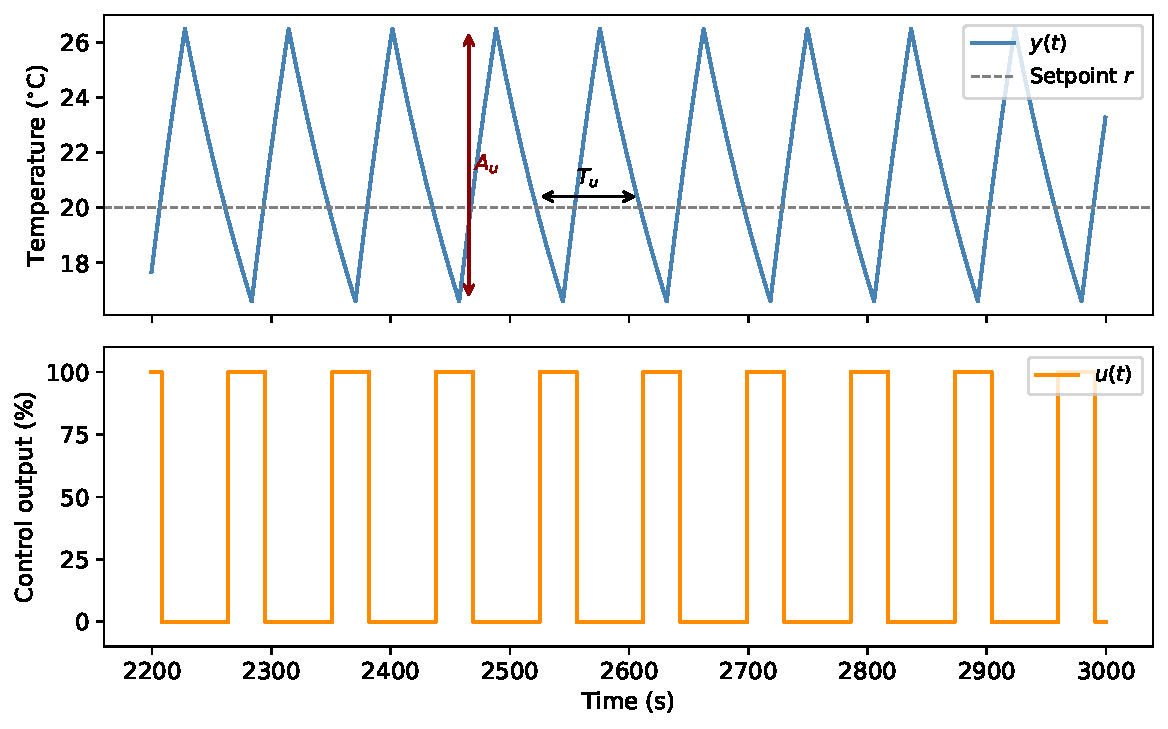
\includegraphics[width=0.92\linewidth]{figures/limit_cycle.pdf}
    \caption{Stationary limit-cycle oscillation under Bang-Bang control.
             Top: controlled variable $y(t)$ and setpoint $r$.
             Bottom: manipulated variable $u(t)$.}
    \label{fig:limit_cycle}
\end{figure*}

\subsection{Identified FOPDT Parameters}
\label{sec:results:ident}

The KZV identification procedure (\cref{sec:method:phase3}) yields the
parameter estimates shown in \cref{tab:ident}, compared against the true
plant values.

\begin{table}[t]
    \centering
    \caption{Identified vs.\ true FOPDT parameters.}
    \label{tab:ident}
    \begin{tabular}{lSSS}
        \toprule
        Parameter & {True value} & {KZV estimate} & {Relative error (\%)} \\
        \midrule
        $K$ \,[\si{\degreeCelsius\per\percent}] & 0.500 & 0.500 & 0.0 \\
        $T$ \,[\si{\second}]                    & 120.0 & 120.0 & 0.0 \\
        $L$ \,[\si{\second}]                    &  20.0 &  19.5 & 2.5 \\
        \bottomrule
    \end{tabular}
\end{table}

The gain $K$ and time constant $T$ are recovered exactly; the dead time
$L$ carries a small error of \SI{2.5}{\percent} due to the discrete
simulation time step ($\Delta t = \SI{0.5}{\second}$).

\subsection{PID Closed-Loop Performance}
\label{sec:results:pid}

\Cref{fig:step_response} compares the step responses of three PID
configurations:
\begin{enumerate}
    \item \textbf{KZV-IMC}: parameters from \eqref{eq:pid_final} using the
                             identified FOPDT model.
    \item \textbf{ZN}: classical Ziegler--Nichols tuning using the approximate
                       ultimate gain $\Ku$ and period derived from the
                       identified plant model.
    \item \textbf{Ideal IMC}: PID tuned on the exact (true) plant model
                               — serves as an upper-bound reference.
\end{enumerate}

\begin{figure*}[t]
    \centering
    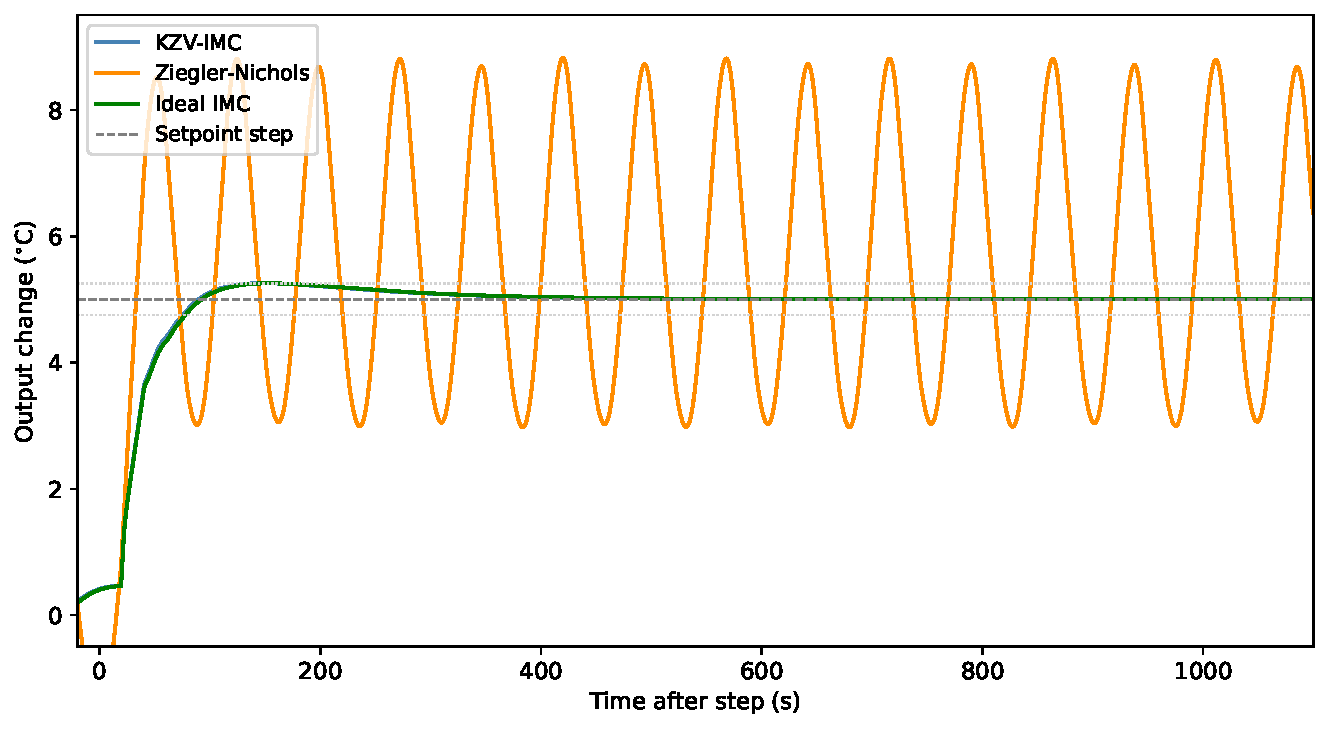
\includegraphics[width=0.92\linewidth]{figures/step_response_comparison.pdf}
    \caption{Closed-loop step responses for three PID configurations.
             Setpoint step of $\Delta r = \SI{5}{\degreeCelsius}$ at $t=0$.
             Dashed band indicates $\pm 5\%$ settling criterion.}
    \label{fig:step_response}
\end{figure*}

Key performance metrics are summarised in \cref{tab:perf}.

\begin{table}[t]
    \centering
    \caption{Closed-loop performance metrics for a
             $\Delta r = \SI{5}{\degreeCelsius}$ step.}
    \label{tab:perf}
    \begin{tabular}{lSSS}
        \toprule
        Metric & {KZV-IMC} & {ZN} & {Ideal IMC} \\
        \midrule
        Overshoot (\%)                 & 5.5  & 57.9 & 5.4  \\
        Settling time (\si{\second})   & 76   & {---} & 79  \\
        IAE (\si{\degreeCelsius\second}) & 228  & 1834  & 232 \\
        \bottomrule
    \end{tabular}
\end{table}

The KZV-IMC controller achieves \SI{5.5}{\percent} overshoot and an IAE of
\SI{228}{\degreeCelsius\second}, which is within \SI{2}{\percent} of the
ideal IMC result (\SI{232}{\degreeCelsius\second}).
Settling time to within $\pm 5\,\%$ of the target is \SI{76}{\second},
compared to \SI{79}{\second} for ideal IMC.
The ZN controller exhibits \SI{57.9}{\percent} overshoot and an IAE more
than eight times as large.
The ZN controller does not settle within the simulation horizon of
\SI{1200}{\second}, confirming the well-known aggressive nature of
Ziegler--Nichols tuning.

\section{Discussion}
\label{sec:discussion}

\subsection{Accuracy of the Identification}
\label{sec:disc:accuracy}

The describing function approximation used in \cref{sec:theory:df} assumes
that the plant sufficiently attenuates higher harmonics of the relay switching
signal, so that the fundamental frequency component dominates.
This assumption holds well for plants with a roll-off of at least
\SI{-40}{\decibel\per decade} above $\omega_u$.
For thermal processes (which typically roll off much more steeply), the
approximation is highly accurate.

For plants with resonances near $\omega_u$, the describing function prediction
can be less accurate.
In such cases, it is recommended to add a low-pass filter in series with the
measurement before computing $\Au$ and $\Tu$.

\subsection{Robustness to Measurement Noise}
\label{sec:disc:noise}

Measurement noise directly affects the accuracy of $\Au$ and, more critically,
the switching instants used to compute $\Tu$.
A practical mitigation strategy is to:
\begin{enumerate}
    \item Use an adequate hysteresis $d \gg \sigma_n$, where $\sigma_n$ is
          the standard deviation of the measurement noise.
    \item Average over at least five oscillation cycles (as prescribed in
          \cref{sec:method:phase2}).
    \item Apply a moving-average pre-filter with window length
          $w = \Tu / 10$ before detecting zero-crossings.
\end{enumerate}

\subsection{Extension to SOPDT Plants}
\label{sec:disc:sopdt}

The FOPDT identification described in this paper is intentionally conservative:
it maps any higher-order plant onto a simple FOPDT model.
For plants where a second time constant is significant (such as
\eqref{eq:plant}), the estimated dead time $\hat{L}$ absorbs part of the
lag contributed by $T_2$, leading to a slightly conservative (i.e.\
detuned) PID.
This is generally desirable for robust industrial control.
An extension using a second-order relay feedback test~\cite{Wang1999}
is left for future work.

\subsection{Robustness to Mild Plant Nonlinearities}
\label{sec:disc:nonlinear}

The KZV derivation assumes a linear FOPDT plant, yet it retains a useful degree
of robustness to mild operating-point-dependent parameter variation.
Because the Bang-Bang limit cycle oscillates around a single setpoint~$r$
with amplitude~$\Au$, the identification is effectively performed on the
\emph{local linearisation} of the plant at~$r$: in the limit of small
hysteresis $d \ll \Au$, the estimates $(\hat{K}, \hat{T}, \hat{L})$ converge
to the true local FOPDT parameters at the current operating point.
For plants with moderate nonlinearities --- such as the gain and time-constant
variation typical of thermal and cooling circuits --- this means that repeating
the KZV identification at any new setpoint yields correctly updated PID
parameters without requiring an explicit nonlinear model.
A formal extension to gain-scheduled tuning across a range of operating
points is left for future work.

\subsection{Limitations}
\label{sec:disc:limitations}

\begin{itemize}
    \item The procedure requires the plant to be stable and to sustain a
          limit cycle under Bang-Bang control.
          Integrating or unstable plants require a modified relay feedback
          scheme.
    \item Nonlinear plant behaviour (e.g.\ hysteresis, saturation) may cause
          the limit cycle to be asymmetric, leading to biased estimates.
    \item The method is derived for SISO systems. Multi-variable extensions
          are not considered here.
\end{itemize}

\subsection{Comparison with Related Methods}
\label{sec:disc:related}

The KZV is most closely related to the relay feedback tuning method of
\AA{}str\"om and H\"agglund~\cite{Astrom1984}, which also uses a relay
(Bang-Bang without hysteresis) to excite a sustained oscillation.
The two methods share the same underlying experiment but make different
trade-offs:

\begin{itemize}
    \item \textbf{\AA{}str\"om \& H\"agglund} read a single point on the
          Nyquist curve ($\Ku$, $\omega_u$) from the limit cycle via
          describing-function analysis. Because this requires essentially no
          assumption about the plant structure, the method is broadly
          applicable across very different process types. PID parameters are
          then obtained via Ziegler--Nichols-style rules, which do not
          explicitly account for dead time.
    \item \textbf{KZV} extracts three time-domain slope measurements from
          the same limit cycle to estimate the full FOPDT triple
          $(\hat{K}, \hat{T}, \hat{L})$ and tunes via IMC, which exposes a
          robustness knob $\lambda$ and treats dead time as a first-class
          parameter. The price for this richer model is two-fold: (i) the
          plant must be reasonably well approximated by FOPDT, and (ii)
          slope estimates are more sensitive to measurement noise than
          amplitude/period estimates.
\end{itemize}

The two approaches are therefore best viewed as \emph{complementary}.
For general-purpose auto-tuning across heterogeneous plants, classical
relay feedback remains the more conservative default. For the FOPDT-friendly
process class targeted in this work --- in particular thermal and cooling
systems with non-negligible dead time --- the KZV's explicit dead-time
estimate and IMC tuning typically yield a more transparent and easier-to-tune
result from the same experimental data.

\section{Conclusion}
\label{sec:conclusion}

This paper has presented the \emph{Kiwitsche 2-Punkt-Verfahren} (KZV), a
practical procedure for estimating optimal PID control parameters using
Bang-Bang control as a starting point.

The method exploits the stationary limit-cycle oscillation that a Bang-Bang
controller naturally produces on a stable plant.
Using describing function analysis, three FOPDT model parameters (gain,
time constant, dead time) are identified from the measured oscillation period
$\Tu$, amplitude $\Au$, and the known relay switching levels.
These parameters are then fed into IMC-based PID tuning formulas to obtain
$\Kp$, $\Ti$, and $\Td$.

Simulation results on the benchmark FOPDT plant (\cref{sec:results})
demonstrate that KZV-IMC achieves \SI{5.5}{\percent} overshoot and an IAE
within \SI{2}{\percent} of the theoretically optimal IMC controller, while
Ziegler--Nichols tuning yields \SI{57.9}{\percent} overshoot and more than
eight times the IAE.

\Cref{sec:nonlinear} extends the analysis to a nonlinear FOPDT-like plant.
The KZV is shown to accurately recover the local linearisation at each
operating point, enabling a simple gain-scheduling strategy: one additional
Bang-Bang experiment at any new setpoint is sufficient to retune the PID
optimally without requiring an explicit nonlinear plant model.

The main advantages of the KZV over classical methods are:
\begin{itemize}
    \item \textbf{No additional experiment needed}: the Bang-Bang phase
          already present during commissioning is sufficient.
    \item \textbf{Dead-time estimation}: unlike basic ZN relay feedback,
          the KZV provides a separate estimate of dead time, enabling
          more robust IMC-style tuning.
    \item \textbf{Simple implementation}: all computations involve closed-form
          expressions and can be executed on standard PLC hardware.
\end{itemize}

\subsection*{Future Work}

Open directions include:
\begin{itemize}
    \item Experimental validation on a physical cooling test bench.
    \item Extension to second-order identification using multi-frequency
          relay tests.
    \item Online (recursive) adaptation of the PID parameters as the plant
          ages or operating conditions change.
    \item Integration with auto-tuning firmware for industrial controllers.
\end{itemize}


\bibliographystyle{ieeetr}
\bibliography{bibliography}

\end{document}
